\documentclass[11pt]{article}
\usepackage{amsmath,textcomp,amssymb,geometry,graphicx,tikz,cancel}
\usepackage{algpseudocode,algorithm}
\usetikzlibrary{trees}
\usepackage[T1]{fontenc}

\def\Name{Zackery Field}  % Your name
\def\Sec{Di, 103}  % Your GSI's name and discussion section
\def\Login{cs170-fe} % Your login
\def\Homework{8}%Number of Homework
\def\Session{Fall 2013}

\title{CS170  Fall 2013 Solutions to Homework 8}
\author{\Name, section \Sec, \texttt{\Login}}
\markboth{CS170 --\Session\  Homework \Homework\ \Name, section \Sec}
{CS170--\Session\ Homework \Homework\ \Name, section \Sec, \texttt{\Login}}
\pagestyle{myheadings}

\begin{document}
\maketitle

\section*{1. (10 pts.) Longest path in a tree}

Give a linear time algorithm that, given an undirected tree $T = (V,E)$ with edges weights
$(w_e)_{e \in E}$, returns the weight of the heaviest path in $T$.


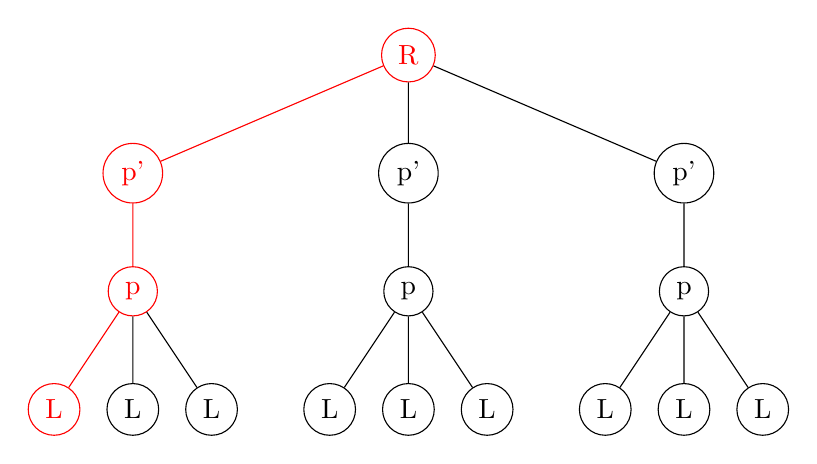
\begin{tikzpicture}[level distance=1.5cm,
level 1/.style={sibling distance=3.5cm},
level 2/.style={sibling distance=1cm}]
\tikzstyle{every node}=[circle,draw]
    \node (Root) [red] {R}
        child [red] {
        node{p'}
        child{
          node {p}
          child { node {L} }
          child [black] { node {L} }
          child [black] { node {L} }
    }}
    child {
      node{p'}
      child{
        node {p}
        child { node {L} }
        child { node {L} }
        child { node {L} }
    }}
    child {
      node{p'}
      child{
        node {p}
        child { node {L} }
        child { node {L} }
        child { node {L} }
        }};

   % Comments to each level
%   \begin{scope}[every node/.style={right}]
%     \path (Root    -| Root-3-3) ++(30mm,0) node {} ++(5mm,0) node 
%     {1};
%     \path (Root-1  -| Root-3-3) ++(30mm,0) node {} ++(5mm,0) node 
%     {$\vdots$};
%     \path (Root-1-1-| Root-3-3) ++(30mm,0) node {} ++(5mm,0) node 
%     {n};
%   \end{scope}

\end{tikzpicture}

For some tree $T$ with root $R$, and leaf vertices $L$. Let $p$ be the parent 
of a given set of leaf vertices and $p'$ be the parent of vertex $p$.
Choose the largest edge weight $p-L_i$ and update the value of 
$p'-p$ to: $(p'-p)=(p'-p)+\mbox{max}\{\forall_i p-L_i\}$. 

The smallest subproblems are the set of vertices $p$ s.t. each $p_i$ is 
the parent of a leaf vertex. We can preprocess the vertices $V$ (in an adjacency
list) and determine the set of nodes $p$ that satisfy the above 
condition by looking collecting the immediate parents of all of the leaf
nodes in a new set $H$. 

     


\label{pg:end-of-p1}
% Make sure that the solution here does not exceed one page here. If
% it does, use the extra space for this problem at the end.  
%
% Comment out the next line if you are NOT using the extra space
 \paragraph{} \emph{Continued on Page \pageref{pg:p1-continuation}}

\newpage

%%Do NOT remove/comment the next line
\pagestyle{plain}
%%It makes sure your name appears only on the first page

\section*{2.  (10 pts.) Problem 7.2, Mathewheatical modeling}

Duckwheat is produced in Kansas and Mexico and consumed in New York and California.
Kansas produces 15 shnupells of duckwheat and Mexico 8. Meanwhile, New York consumes
10 shnupells and California 13. The transportation costs per shnupell are \$4 from Mexico to
New York, \$1 from Mexico to California, \$2 from Kansas to New York, and \$3 and from Kansas
to California. Write a linear program that decides the amounts of duckwheat (in shnupells
and fractions of a shnupell) to be transported from each producer to each consumer, so as to
minimize the overall transportation cost.

\begin{equation*}
  \begin{aligned}
    %x_k=Kansas,x_m=Mexico,x_n=New\:York,x_c=California\\
    p_{k,n}=\mbox{Kansas to New York}=\$2 &,p_{k,c}=\mbox{Kansas to California}= \$3\\
    p_{m,n}=\mbox{Mexico to New York}=\$4 &,p_{m,c}=\mbox{Mexico to California}= \$1\\
    x_{k,n}=\mbox{amt form Kansas to New York}&,x_{k,c}=\mbox{amt form Kansas to California}\\
    x_{m,n}=\mbox{amt form Mexico to New York}&,x_{m,c}=\mbox{amt form Mexico to California}\\
    %y_k=Kansas,y_m=Mexico,y_n=New\:York,y_c=California\\
  \end{aligned}
\end{equation*}

\begin{equation*}
  \begin{aligned}
    \mbox{min: } x_{k,n}p_{k,n} &+x_{k,c}p_{k,c} +x_{m,n}p_{m,n} +x_{m,c}p_{m,c}\\
    x_{k,n}&+x_{k,c} \leq 15 \\
    x_{m,n}&+x_{m,c} \leq 8  \\
    x_{k,n}&+x_{m,n} \geq 10 \\
    x_{k,c}&+x_{m,c} \geq 13 \\
  \end{aligned}
\end{equation*}

\label{pg:end-of-p2}
% Make sure that the solution here does not exceed one page here. If
% it does, use the extra space for this problem at the end.  
%
% Comment out the next line if you are NOT using the extra space
% \paragraph{} \emph{Continued on Page \pageref{pg:p2-continuation}}

\newpage

\section*{3. (10 pts.) Problem 7.7, A feasibility study}

Find necessary and sufficient conditions on real numbers $a$ and $b$ under which
the linear program 

\begin{equation*}
  \begin{aligned}
    \mbox{max: } x+y&\\
    ax + by &\leq 1\\
    x,y &\geq 0
  \end{aligned}
\end{equation*}

Assume that $x,y\in \mathbb{R}$

y-intercept: $1/b$

x-intercept: $1/a$

\begin{itemize}
\item[(a)] Is infeasible.

Since both $x$ and $y$ could be $0$, for any choice of $a$ and $b$, 
$a*0+b*0\leq 1$. Therefore, no choice of $a$ and $b$ exists that makes
the solution to max: $x+y$ infeasible. 

\item[(b)] Is unbounded.

$a\leq 0 \vee b\leq 0$. Let $(-)$ denote some nonpositive number, and $(+)$ 
denote some nonnegative number, these possible scenarios occur


\begin{equation}
  \begin{aligned}
    (-)x + (-)y &\leq 1\\
    (+)x + (-)y &\leq 1\\
    (-)x + (+)y &\leq 1\\
  \end{aligned}
\end{equation}

For equation (1) any choice of $x$ and $y$ will satisfy the inequality.
For equation (2), holding $x$ at some value that satisfies the inequality will
allow $y$ to be any number, making the solution unbounded.
Equivalently, for equation (3), holding $y$ at some value that satisfies the inequality will
allow $x$ to be any number, making the solution unbounded.

\item[(c)] Has a unique and optimal solution.

 $a>0 \wedge b>0$. As before, let $(-)$ denote some nonpositve number, and $(+)$
denote some nonnegative number. There is only one possible configuration in this
case $(+)x + (+)y \leq 1$. Since there is a nonnegative constraint on
$x$ and $y$, then there is some constraint on the maximum values of $x$ and $y$, 
Per the argument in the infeasibility section, there is no choice of $a$ and
$b$ that would be small enough to make the solution unbounded. 

\end{itemize}


 
\label{pg:end-of-p3}

% Make sure that the solution here does not exceed one page here. If
% it does, use the extra space for this problem at the end.  
%
% Comment out the next line if you are NOT using the extra space
% \paragraph{} \emph{Continued on Page \pageref{pg:p3-continuation}}

\newpage

\section*{4.  (10 pts.) Problem 7.12, Provably optimal}

For a linear program

\begin{equation*}
  \begin{aligned}
    \mbox{max: } x_1-2x_3\\
    x_1-x_2 &\leq 1\\
    2x_2-x_3 &\leq 1\\
    x_1,x_2,x_3 & \geq 0\\
  \end{aligned}
\end{equation*}

Show that the solution $(x_1,x_2,x_3)=(3/2,1/2,0)$ is optimal.

To show that this solution is optimal I will construct a dual LP and show that
it has the same optimal value $x_1-2x_3=3/2-2*0=3/2$.

{
  \centering
  \begin{tabular}{c | c}
    Multiplier & Inequality\\
    $y_1$ & $x_1-x_2 \leq 1$\\
    $y_2$ & $2x_2-x_3 \leq 1$\\
  \end{tabular}\par
}

\begin{equation*}
  \begin{aligned}
    (y_1)(x_1-x_2) + (y_2)(2x_2-x_3) &\leq y_1+y_2\\
    (y_1)x_1+(2y_2-y_1)x_2-(y_2)x_3 & \leq y_1+y_2
  \end{aligned}
\end{equation*}

\begin{equation*}
  \begin{aligned}
    &x_1-2x_3 \leq y_1+y_2 \mbox{ if } \left\{  
      \begin{array}{lr}
        y_1,y_2 &\geq 0 \\
        y_1 &\geq 1 \\
        2y_2-y_1 &\geq 0\\
        y_2 &\geq -2 \\
      \end{array}
    \right. 
   \end{aligned}
\end{equation*}

\begin{equation*}
  \begin{aligned}
    \mbox{min: }y_1+y_2&\\
    y_1,y_2 &\geq 0 \\
    y_1 &\geq 1 \\
    2y_2-y_1 &\geq 0\\
    y_2 &\geq -2 \\
  \end{aligned}
\end{equation*}

By inspection, the maximum solution to this dual LP is $(y_1,y_2)=(1,1/2)\Rightarrow 3/2$.
By the duality theorem, the primal (given) LP and the dual LP both have the same optimum value, 
which gurantees that the given solution $(x_1,x_2,x_3)=(3/2,1/2,0)$ is optimal.

\label{pg:end-of-p4}

% Make sure that the solution here does not exceed one page here. If
% it does, use the extra space for this problem at the end.  
%
% Comment out the next line if you are NOT using the extra space
% \paragraph{} \emph{Continued on Page \pageref{pg:p4-continuation}}


\newpage

\section*{5. (10 pts.) Problem 7.9, Non-linear programming}

A quadratic programming problem seeks to maximize a quadratric objective function 
(with terms like $3x_1^2,5x1x2$ ) subject to a set of
linear constraints. Give an example of a quadratic program in two variables 
$x_1$, $x_2$ such that the feasible region is nonempty and bounded, and yet 
none of the vertices of this region optimize the (quadratic) objective.
\newline
\newline
$f(x_1,x_2)=  -x_1^2 -x_2^2$, subject to constraints 

\begin{equation*}
  \begin{aligned}
    x_1 &\geq -1/2\\
    x_2 &\geq -1/2\\
    x_2-x_1 &\leq 1
  \end{aligned}
\end{equation*}

The maximum of $f(x_1,x_2)$ is at $f(0,0)=0$. The 3 constraints form a triangle 
that intersects with the point $(x_1,x_2,f(x_1,x_2))=(0,0,0)$, but not 
at a vertex of the triangle.

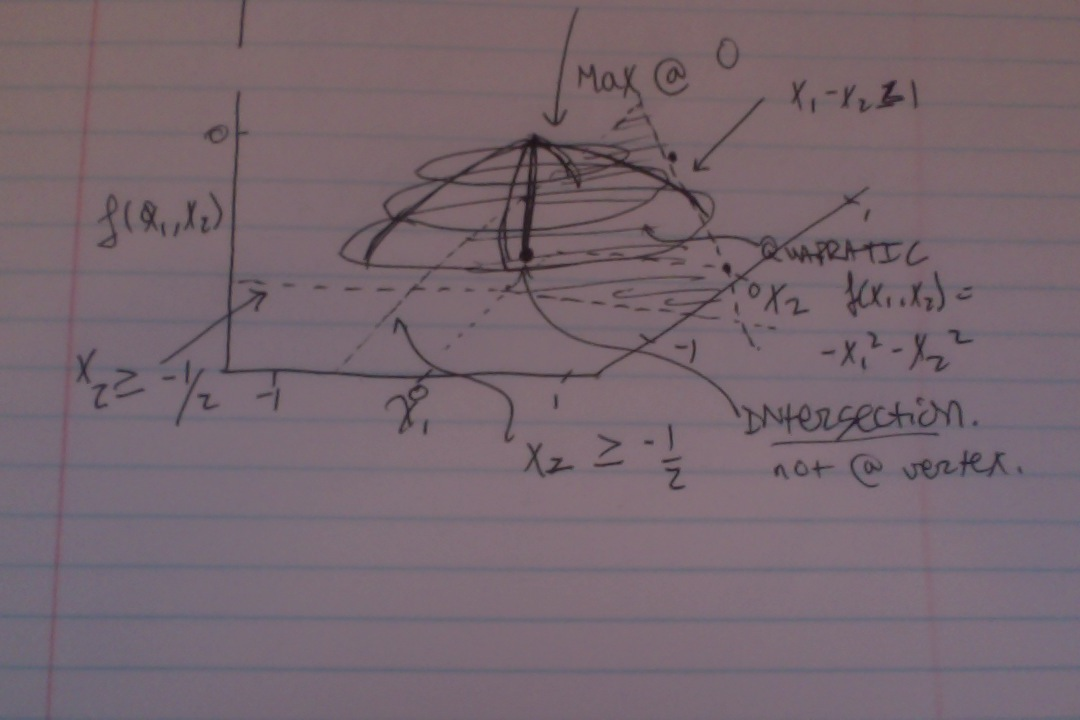
\includegraphics[scale=0.4]{ps9_graph.jpg}

\label{pg:end-of-p5}


% Make sure that the solution here does not exceed one page here. If
% it does, use the extra space for this problem at the end.  
%
% Comment out the next line if you are NOT using the extra space
% \paragraph{} \emph{Continued on Page \pageref{pg:p5-continuation}}

\newpage


 \section*{6. (10 pts.) Problem 7.21, Flows through cuts}

An edge of an $s-t$ flow network is called \emph{critical} if decreasing the 
capacity of this edge results in a decrease in the $s-t$ maximum flow. 
Give an efficient algorithm that finds a critical edge in a network.
-
Run the max-flow algorithm on the given network (takes $O(|V||E|^2)$ time p. 203 in txt).
By the max-flow min-cut theorem, the max-flow algorithm will return the minimum
(s,t)-cut (see p.202 in text). This cut defines the maximum flow capacity.
Any edge in the minimum (s,t)-cut with positive capacity ($s\rightarrow t$ directionality)
will be a critical edge, because the reduction of this edge's capacity will
reduce the maximum possible flow from $s-t$. Proof: see section 7.2 in the text.

Runtime of max-flow defined in p.203 of the text: $O(|V||E|^2)$.

\label{pg:end-of-p6}

% Make sure that the solution here does not exceed one page here. If
% it does, use the extra space for this problem at the end.  
%
% Comment out the next line if you are NOT using the extra space
%\paragraph{} \emph{Continued on Page \pageref{pg:p6-continuation}}

\newpage


% Comment out the "extra spaces" completely for the problems for you
% don't neethem
 
 \section*{Extra space for Problem 1}
 \emph{Continued from Page \pageref{pg:end-of-p1}}
 

 \label{pg:p1-continuation}

Starting with the list $H$ and moving upward through the tree always updating 
the edge  $v'-v$ ($v'$ is the parent of $v$) with the maximum of the edge weights
of all of the paths $v-v_{children}$. This will lead to the heaviest weight path
being stored in one of the edges connecting the root to its children. To return the
actual path that led to this heaviest path, start by assuming that all edge weights are
distinct, and then simply follow the edges downward the tree by maximum value back to a leaf
node. 

Proof by induction: The base case is the set of vertices $H$. Take one of these
vertices $p$. If we want to find the maximum edge weight extending from $p$, then
we can trivially observe the largest edge weight extending from $p$ to its children
(which are leaf nodes). 
Let $v$ be some arbitrary vertex, with parent $v'$, and children $v_c$.
We can hypothesize that all vertices $v-v_c$ have been updated with the maximum
edge weights to each $v_c$. 
It follows that the process of updating the edge $v'-v$ with the maximum of the
weights $v-v_c$ will require that $v'-v$ now contains the maximum edge weight path.

The preprocessing of the grpah to find the set of vertices $H$, where each vertex in
$H$ only has leaf vertex children, takes linear time.
Since each path is looked at exactly once in order to find the maximum, and then
the parent path is updated once at most for each parent edge, then the total running
time is linear; $O(|V|+|E|)$.
 
 
% \newpage
 %%Comment out the above three lines if you are not using extraspace
 %%for this problem.
 
 
 %\section*{Extra space for Problem 2}
 %\emph{Continued from Page \pageref{pg:end-of-p2}}
 %  
 %\label{pg:p2-continuation}
% %\newpage
% %%Comment out the above three lines if you are not using extra space
% %%fo: r this problem.
% 
: % \: section*{Extra space for Problem 3}
% \: emph{Continued from Page \pageref{pg:end-of-p3}}
% 
% \label{pg:p3-continuation}
%
%\newpage
%Comment out the above three lines if you are not using extra space
%for this problem.
 
% \section*{Extra space for Problem 4}
% \emph{Continued from Page \pageref{pg:end-of-p4}}
% 
% 
% \label{pg:p4-continuation}
% \newpage
 %%Comment out the above three lines if you are not using extra space
 %%for this problem.
 
 
% \section*{Extra space for Problem 5}
% \emph{Continued from Page \pageref{pg:end-of-p5}}
% 
% \label{pg:p5-continuation}
% \newpage
 %%Comment out the above three lines if you are not using extra space
 %%for this problem.
%
% \section*{Extra space for Problem 6}
%% \emph{Continued from Page \pageref{pg:end-of-p6}}
%%%% 
% 
% %Insert solution here
%%%% 
% 
% \label{pg:p6-continuation}
% \newpage
%%Comment out the above three lines if you are not using extra space
%%for this problem.



% \begin{tikzpicture}[level/.style={sibling distance=40mm/#1}]
% \node (z){$A$}
% child {node (a) {}
%     child {node  (b) {}
%       child {node (b1) {$\vdots$}
%        child {node (b11) {$D$}}
%       }
%       child {node (b2) {$\vdots$}
%        child {node (b12) {$D$}}
%       }
%     }
%     child {node (g) {}
%       child {node (g1) {$\vdots$}
%        child {node (g11) {$D$}}
%       }
%       child {node (g2) {$\vdots$}
%        child {node (g12) {$D$}}
%       }
%     }
%   }
%     child {node (d) {}
%       child {node  (e) {}
%         child {node (e1) {$\vdots$}
%          child {node (e11) {$D$}}
%         }
%         child {node (e2) {$\vdots$}
%          child {node (e12) {$D$}}
%         }
%       }
%       child {node (f) {}
%         child {node (f1) {$\vdots$}
%          child {node (f11) {$D$}}
%         }
%         child {node (f2) {$\vdots$}
%          child {node (f12) {$D$}}
%         }
%       }
%     }
%   child {node  (j) {}
%     child {node (k) {}
%       child {node {$\vdots$}
%        child {node (k11) {$D$}}
%       }
%       child {node {$\vdots$}
%        child {node (k12) {$D$}}
%       }
%     }
%     child {node (l) {}
%     child {node {$\vdots$}
%      child {node (l11) {$D$}}
%     }
%     child {node (c){$\vdots$}
%      child {node (l12) {$D$}
%             child [grow=right] {node (r) {$n$} edge from parent[draw=none]
%               child [grow=up] {node (s) {$\vdots$} edge from parent[draw=none]
%                 child [grow=up] {node (t) {$n$} edge from parent[draw=none]
%                   child [grow=up] {node (u) {$n$} edge from parent[draw=none]
%                    child [grow=up] {node (u) {$n$} edge from parent[draw=none]}
%                   }
%                 }
%               }
%             }
%             }
%     }
%   }
% };
% \path (b) -- (g) node [midway] {$\cdots$};
% \path (e) -- (f) node [midway] {$\cdots$};
% \path (k) -- (l) node [midway] {$\cdots$};
% \path (b11) -- (b12) node [midway] {$\cdots$};
% \path (g11) -- (g12) node [midway] {$\cdots$};
% \path (e11) -- (e12) node [midway] {$\cdots$};
% \path (f11) -- (f12) node [midway] {$\cdots$};
% \path (k11) -- (k12) node [midway] {$\cdots$};
% \path (l11) -- (l12) node [midway] {$\cdots$};
% \end{tikzpicture}

\end{document}
